\documentclass[11pt]{article}
\usepackage[T1]{fontenc}
\usepackage{lmodern}
\usepackage[margin=1in]{geometry}
\usepackage{amsmath,amssymb,amsthm}
\usepackage{microtype}
\usepackage{flafter}
\usepackage{enumitem}
\usepackage{xcolor}
\usepackage{tikz}
\usetikzlibrary{arrows.meta,positioning}
\usepackage[colorlinks=true,linkcolor=blue!45!black,citecolor=blue!45!black,urlcolor=blue!45!black]{hyperref}
\hypersetup{pdftitle={A superquadratic separation between sensitivity and block sensitivity},pdfauthor={Rewritten for readability from the OpenAI manuscript of the same title}}
\newcommand{\bs}{\operatorname{bs}}
\newcommand{\dist}{\operatorname{dist}}
\newcommand{\unverified}[1]{\par\smallskip\noindent\fbox{\parbox{0.95\linewidth}{\textbf{Unverified step.} #1}}\par\smallskip}
\newtheorem{theorem}{Theorem}[section]
\newtheorem{lemma}[theorem]{Lemma}
\newtheorem{proposition}[theorem]{Proposition}
\newtheorem{corollary}[theorem]{Corollary}
\theoremstyle{definition}
\newtheorem{definition}[theorem]{Definition}
\theoremstyle{remark}
\newtheorem{remark}[theorem]{Remark}
\title{A superquadratic separation between sensitivity\\and block sensitivity}
\author{Rewritten for readability from the OpenAI manuscript of the same title}
\date{September 25, 2026}
\begin{document}
\maketitle
\begin{abstract}
We disprove the quadratic strengthening of the Sensitivity Conjecture by
constructing nonconstant total Boolean functions whose block sensitivity
exceeds any prescribed constant multiple of sensitivity squared
(Theorem~\ref{thm:main}). Composing one such function with itself then gives,
for some fixed \(\alpha>2\), a sequence of functions \(F_\nu\) with unbounded
block sensitivity and
\(\bs(F_\nu)\ge\bs(F_\nu,0)\ge s(F_\nu)^\alpha\)
(Corollary~\ref{cor:power-separation}).
\end{abstract}

\section{Results, context, and the proof at a glance}
\label{sec:introduction}

\subsection{Definitions and statements}

For a positive integer \(n\), write \([n]=\{1,\ldots,n\}\).
A \emph{total Boolean function} is a map \(f:\{0,1\}^n\to\{0,1\}\) defined on
every input.
If \(x\in\{0,1\}^n\) and \(B\subseteq[n]\), let \(x^B\) be the string obtained
from \(x\) by flipping exactly the coordinates in \(B\); abbreviate
\(x^{\{e\}}\) to \(x^e\). We write \(0\) for the all-zero string, so \(0^B\)
is the indicator string of \(B\).

The \emph{sensitivity} of \(f\) is
\[
 s(f,x)=\bigl|\{e\in[n]:f(x^e)\ne f(x)\}\bigr|,
 \qquad s(f)=\max_x s(f,x).
\]
A \emph{sensitive block for \(f\) at \(x\)} is a nonempty set \(B\subseteq[n]\)
with \(f(x^B)\ne f(x)\). The \emph{block sensitivity} \(\bs(f,x)\) is the
largest number of pairwise disjoint sensitive blocks for \(f\) at \(x\), and
\(\bs(f)=\max_x\bs(f,x)\). In particular \(\bs(f)\ge\bs(f,0)\).

\begin{theorem}\label{thm:main}
For every real \(C>0\), there are a positive integer \(n\) and a
nonconstant total Boolean function \(f:\{0,1\}^n\to\{0,1\}\) such that
\[
 \bs(f)>C\,s(f)^2.
\]
More precisely, for every integer \(d\ge1\) the construction below gives
a nonconstant total Boolean function \(f\) with
\[
 \frac{\bs(f)}{s(f)^2}\ge \frac{2^d}{4(d+2)^2}.
\]
\end{theorem}

\begin{corollary}\label{cor:power-separation}
There exist a real number \(\alpha>2\) and nonconstant total Boolean
functions \(F_\nu\), for integers \(\nu\geq1\), such that
\[
 \bs(F_\nu,0)\geq s(F_\nu)^\alpha
 \qquad\text{for every }\nu,
 \qquad
 \bs(F_\nu,0)\longrightarrow\infty .
\]
\end{corollary}

\paragraph{What the proofs deliver concretely.}
For every \(d\ge1\) and every integer \(M\ge9^{d+1}\) we construct an explicit
\(f\) (up to the choice of a labelling whose existence is shown
probabilistically) with \(f(0)=0\),
\[
 s(f)\le 2(d+2)M^{d+1},\qquad \bs(f,0)\ge M^2(2M^2+1)^d ;
\]
see \eqref{eq:final-sensitivity} and \eqref{eq:final-block-sensitivity}.
The bound \(2^d/(4(d+2)^2)\) is below \(1\) for \(d\le 8\) and equals
\(512/484\) at \(d=9\); this is why the Corollary uses the seed \(d=9\).
The exponent \(\alpha\) of the Corollary is \(\log B/\log A\) for two numbers
\(A,B\) depending on the chosen \(M\ge 9^{10}\); it is fixed once \(M\) is
fixed, it is not canonical, and it is only slightly larger than \(2\).

\subsection{Context (not used in the proofs)}

This subsection reproduces the source's background and attributions. It was
not checked against the cited papers, and no statement in it is used in the
proofs, which are self-contained.

The Sensitivity Conjecture asked whether block sensitivity is bounded by a
polynomial in sensitivity, uniformly over the number of inputs and the
function. The question goes back to Nisan's work on parallel computation,
which introduced block sensitivity and already recorded Rubinstein's
quadratic separation \cite[Section~2]{Nisan1989}.
Nisan and Szegedy explicitly suggested the quadratic inequality
\(\bs(f)\le s(f)^2\) \cite[Section~4]{NisanSzegedy1994}.
Rubinstein's construction \cite{Rubinstein1995} showed that a polynomial
upper bound would need degree at least two. Virza improved the separation
to \(\bs(f)=\tfrac12s(f)^2+\tfrac12s(f)\) \cite{Virza2011}, and
Ambainis and Sun obtained
\(\bs(f)=\frac23s(f)^2-\frac13s(f)\) \cite[Theorem~1]{AmbainisSun2011}.
Huang resolved the polynomial conjecture in 2019: his degree bound,
together with Tal's refinement of the degree--block-sensitivity comparison
\cite{Tal2013}, gives \(\bs(f)\le s(f)^4\) for every total Boolean function
\cite[Theorem~1.5]{Huang2019}. Wellens improved the leading constant to
\(\bs(f)\le\sqrt{2/3}\,s(f)^4+1\) \cite[Corollary~4.2]{Wellens2022}.
Theorem~\ref{thm:main} rules out the quadratic strengthening; it does not
conflict with the quartic upper bound, since it only excludes exponent
\(2\).

\emph{Relation to spectral sensitivity.}
According to the source, Meiburg's spectral-sensitivity construction uses
tournament-indexed rows of positive conditions and one selected blocking
coordinate in each outgoing row
\cite[Sections~3.1 and~5.2--5.5]{Meiburg2026}.\footnote{In the
attribution accompanying this construction, Meiburg credits GPT-5.6-Sol
with the gated-tournament ideas and describes his own contributions as
exposition, size and parameter optimization, and checking the faithfulness
of the Lean formalization.}
The present construction adapts that architecture (rows, tournament, one
labelled child per outgoing edge) to \emph{nested} predicates. What is
different, again according to the source, is the forbidden-label condition
(here Lemma~\ref{lem:labelling}, proved by a direct union bound) and the use
of simultaneous changes of two predicates to control ordinary sensitivity.
Nothing from \cite{Meiburg2026} is used as a logical input.
Spectral sensitivity \(\lambda(f)\) is the operator norm of the adjacency
matrix of the graph joining adjacent inputs on which \(f\) differs
\cite{AaronsonEtAl2021}; since \(\lambda(f)\le s(f)\), a lower bound on
\(\bs(f)/\lambda(f)^2\) alone would not give Theorem~\ref{thm:main}.

\emph{Other borrowed principles.} Taking an OR of disjoint copies to balance
the sensitivities at zero-inputs and one-inputs follows Ambainis and Sun
\cite[Section~4, Lemma~1]{AmbainisSun2011}. Ambainis and Pr\={u}sis noted
that a seed with block sensitivity greater than sensitivity squared would
yield a superquadratic power separation by iteration
\cite[Section~1]{AmbainisPrusis2014}; composition as an amplification method
is treated systematically by Tal~\cite{Tal2013}. The two composition facts
we need are proved in Lemma~\ref{lem:composition}.

\subsection{Proof at a glance}
\label{sec:glance}

\paragraph{The object.}
Fix a depth \(d\ge1\) and a size parameter \(M\), and put \(L=d+2\),
\(k=2M^2+1\), \(r=\lceil\sqrt M\rceil\). For each level
\(\ell=0,\ldots,d\) we define a short list of Boolean functions
(``predicates'') on the same \(N_\ell\) bits,
\(P_{\ell,1}\ge P_{\ell,2}\ge\cdots\ge P_{\ell,H_\ell}\) pointwise; this chain
is what ``nested'' means. At level \(0\), \(P_{0,q}\) accepts the inputs
within Hamming distance \(d+1-q\) of one of \(M\) far-apart centres. A
level-\(\ell\) input is cut into \(kr\) level-\((\ell-1)\) inputs
(``children''), arranged in \(k\) rows of \(r\). The rows are the vertices of
a tournament in which every row has exactly \(M^2\) out-neighbours, and each
edge \(i\to j\) carries a label \(a(i,j)\) naming one child of row \(j\).
The predicate \(P_{\ell,q}\) is an OR of \(k\) clauses, one per row.
Clause \(i\) requires:
\begin{itemize}[nosep]
\item \emph{targets}: the strongest (highest-index) child predicate accepts
 all \(r\) children of row \(i\);
\item \emph{gates}: for each of the \(M^2\) edges \(i\to j\), a weaker child
 predicate (which one depends on \(q\)) rejects the labelled child of row
 \(j\).
\end{itemize}
The final function \(f\) is the OR of \(M\) disjoint copies of \(P_{d,1}\).

\paragraph{Why block sensitivity is large (easy).}
At the all-zero input every predicate rejects. Flipping, in every child of
one row, a block that turns that child on satisfies that row's clause: its
targets hold, and its gate children lie in other rows, are untouched, and
still reject. Every one of the \(k\) rows can be used, so the number of
disjoint sensitive blocks at zero is multiplied by \(k=2M^2+1\) per level
(Lemma~\ref{lem:blocks}), giving \(\bs(f,0)\ge M^2k^d\).

\paragraph{Why sensitivity is small (the work).}
Let \(S_{\ell,0}\) (resp.\ \(S_{\ell,1}\)) be the largest number of single-bit
flips that take some \(P_{\ell,q}\) from \(0\) to \(1\) (resp.\ from \(1\) to
\(0\)) at some input. The goal is \(S_{\ell,b}\le 2LM^{\ell+b}\): sensitivity
grows by a factor about \(M\) per level, so \(s^2\) grows by about \(M^2\),
while the block count grows by \(2M^2+1\). The gain is a factor \(2\) per
level.
\begin{itemize}[leftmargin=1.5em]
\item \emph{From \(1\) to \(0\).} Fix one satisfied clause; a flip must break
 one of its \(M^2\) gates or \(r\) targets. Hence
 \(S_{\ell,1}\le M^2S_{\ell-1,0}+rS_{\ell-1,1}\).
\item \emph{From \(0\) to \(1\).} A flip touches one child, and a clause
 tests each child at most once (Lemma~\ref{lem:structure}), so the flip must
 complete a clause that was exactly one condition short. Call
 \(\mathcal T\) the clauses with exactly one failed target, and
 \(\mathcal G\) those with exactly one failed gate. The labels force
 \(|\mathcal T|\le 15\) (Lemma~\ref{lem:labelling}), and each such clause
 costs \(S_{\ell-1,0}\), a lower-order quantity. The tournament forces
 \(|\mathcal G|\le3\). Repairing a failed gate means turning a child
 predicate from \(1\) to \(0\), which may cost \(S_{\ell-1,1}\), the main
 term. Charging \(S_{\ell-1,1}\) to all three clauses would give growth
 \(3M\) per level and destroy the gain. The key observation is that for all
 clauses in \(\mathcal G\) except at most one (the \emph{exceptional}
 clause, defined in Step~C3 of the proof of
 Proposition~\ref{prop:recurrences}), the failed gate sits on a child that
 is a satisfied target of another clause of \(\mathcal G\). There the
 strongest child predicate is \(1\), and by nesting the repair must turn
 \emph{both} the gate predicate and the strongest predicate to \(0\). Such
 flips are counted by a \emph{joint sensitivity} \(J_{\ell-1,1}\), which will
 be tiny. Hence
 \(S_{\ell,0}\le 16\,S_{\ell-1,0}+S_{\ell-1,1}+3J_{\ell-1,1}\).
\item \emph{Controlling \(J\).} \(J_{\ell,b}\) counts flips that change two
 distinct predicates \(P_{\ell,q},P_{\ell,q'}\) together from \(b\) to
 \(1-b\). At level \(0\) it is zero, since one flip changes a Hamming
 distance by at most \(1\) and cannot cross two integer radii
 (Lemma~\ref{lem:base}). It obeys its own recurrences,
 \(J_{\ell,1}\le M^2J_{\ell-1,0}+rS_{\ell-1,1}\) and
 \(J_{\ell,0}\le16\,S_{\ell-1,0}+3J_{\ell-1,1}\). In the last bound even the
 exceptional clause is charged \(J_{\ell-1,1}\): making a clause hold for two
 parent indices \(q<q'\) forces two child gate predicates to change.
\item \emph{Solving the recurrences.} After dividing by \(M^{\ell+b}\), the
 normalised \(S\)-quantity \(u_\ell\) and \(J\)-quantity \(v_\ell\) satisfy
 \(u_\ell\le(1+\epsilon)u_{\ell-1}+3v_{\ell-1}\),
 \(v_\ell\le\epsilon u_{\ell-1}+3v_{\ell-1}\) with
 \(\epsilon\le 2/\sqrt M\). The quantity \(v\) may triple per level, but it
 starts at \(0\) and is fed only by \(\epsilon u\). The hypothesis
 \(M\ge 9^{d+1}\) gives \(\epsilon\,3^{d+1}\le 2\), which keeps
 \(u_\ell\le 2L\) for all \(\ell\le d\)
 (Lemma~\ref{lem:quantitative-profiles}).
\item \emph{Balancing.} \(P_{d,1}\) has \(S_{d,0}\le2LM^{d}\) but
 \(S_{d,1}\le 2LM^{d+1}\). The OR of \(M\) copies has sensitivity at most
 \(\max\{MS_{d,0},S_{d,1}\}\le 2LM^{d+1}\) and \(M\) times as many blocks.
\end{itemize}
Then
\(\bs(f,0)/s(f)^2\ge M^2k^d/(4L^2M^{2d+2})=(k/M^2)^d/(4L^2)\ge2^d/(4L^2)\).

\paragraph{The Corollary.}
For disjoint composition, sensitivity is submultiplicative and block
sensitivity at zero is supermultiplicative (Lemma~\ref{lem:composition}).
Iterating the seed \(d=9\), for which \(\bs(f,0)\ge B>A^2\ge s(f)^2\), gives
\(\bs(F_\nu,0)\ge B^\nu\) and \(s(F_\nu)\le A^\nu\).

\begin{figure}[htbp]
\centering
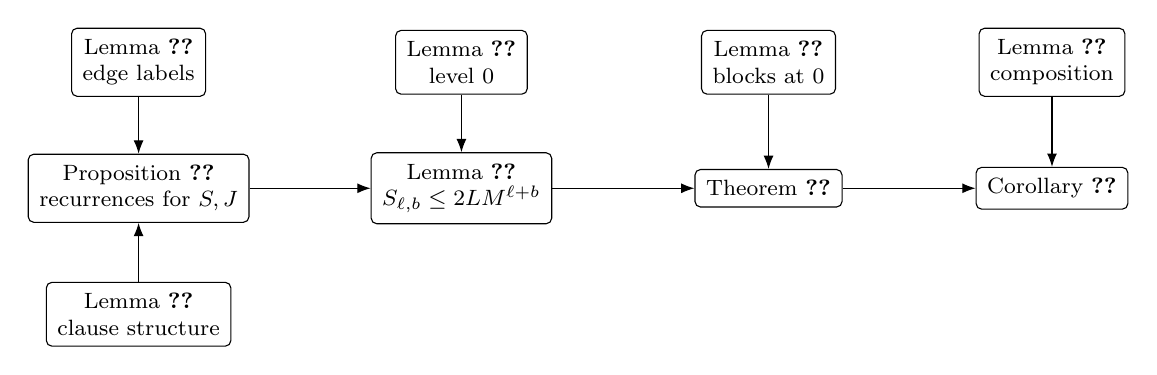
\begin{tikzpicture}[>=Latex, every node/.style={font=\footnotesize},
  box/.style={draw,rounded corners=2pt,inner sep=4pt,align=center}]
 \node[box] (rec) at (0,0) {Proposition~\ref{prop:recurrences}\\recurrences for \(S,J\)};
 \node[box] (quant) at (4.1,0) {Lemma~\ref{lem:quantitative-profiles}\\\(S_{\ell,b}\le2LM^{\ell+b}\)};
 \node[box] (main) at (8.0,0) {Theorem~\ref{thm:main}};
 \node[box] (cor) at (11.6,0) {Corollary~\ref{cor:power-separation}};
 \node[box] (lab) at (0,1.6) {Lemma~\ref{lem:labelling}\\edge labels};
 \node[box] (str) at (0,-1.6) {Lemma~\ref{lem:structure}\\clause structure};
 \node[box] (base) at (4.1,1.6) {Lemma~\ref{lem:base}\\level \(0\)};
 \node[box] (blk) at (8.0,1.6) {Lemma~\ref{lem:blocks}\\blocks at \(0\)};
 \node[box] (comp) at (11.6,1.6) {Lemma~\ref{lem:composition}\\composition};
 \draw[->] (lab) -- (rec);
 \draw[->] (str) -- (rec);
 \draw[->] (rec) -- (quant);
 \draw[->] (base) -- (quant);
 \draw[->] (quant) -- (main);
 \draw[->] (blk) -- (main);
 \draw[->] (main) -- (cor);
 \draw[->] (comp) -- (cor);
\end{tikzpicture}
\caption{Dependencies. An arrow means ``is used in the proof of''.}
\label{fig:dependencies}
\end{figure}

\subsection{Notation, and symbols renamed from the source}
\label{sec:notation}

Each symbol below has one meaning throughout.
\begin{center}
\begin{tabular}{ll}
\(d,\ M,\ L=d+2,\ k=2M^2+1,\ r=\lceil\sqrt M\rceil,\ t=16\) & global parameters\\
\(\ell\); \(H_\ell=d+1-\ell\); \(N_\ell=LM(kr)^\ell\) & level; number of predicates; number of bits\\
\(q<q'\) & predicate indices at the current (parent) level\\
\(H=H_\ell\), \(Q=H+1=H_{\ell-1}\) & shorthand at a fixed level \(\ell\ge1\)\\
\(i,j\in[k]\); \(c\in[r]\); \(a(i,j)\in[r]\) & rows; positions; edge labels\\
\(e\) & a single coordinate (bit) of an input\\
\(S_{\ell,b},\,J_{\ell,b}\); \(S'_b,\,J'_b\) & profiles; the same at level \(\ell-1\)\\
\end{tabular}
\end{center}
To keep one meaning per symbol, the following names differ from the source;
the mathematics is unchanged. Single coordinates are called \(e\) (source:
\(a\), which also names the edge labels). The gate indices are
\(\gamma=Q-q\), \(\gamma'=Q-q'\) (source: \(g,g'\)). The size of
\(\mathcal G\) is written \(|\mathcal G|\) (source: \(m\)). In
Lemma~\ref{lem:composition} the dimensions are \(n_1,n_2\) (source: \(a,b\)),
the outer string is \(w\) (source: \(y\)), the blocks are
\(X_s,Y_{s'}\) (source: \(C_i,D_j\)) and their numbers \(p,p'\) (source:
\(p,q\)). The index in the Corollary is \(\nu\) (source: \(m\)).

\section{The construction}
\label{sec:construction}

\subsection{Parameters and the tournament}

Fix integers \(d\ge1\) and \(M\ge3\), and put
\[
 L=d+2,\qquad k=2M^2+1,\qquad r=\lceil\sqrt M\rceil,
 \qquad t=16.
\]
Sections~\ref{sec:construction}--\ref{sec:recurrences} only need \(M\ge3\);
from Section~\ref{sec:separation} on we assume \(M\ge 9^{d+1}\).

A \emph{tournament} on a vertex set is an orientation of every pair of
distinct vertices: for \(i\ne j\) exactly one of \(i\to j\) and \(j\to i\)
holds. We fix a tournament on \([k]\) in which every vertex has outdegree
exactly \(M^2\). One exists: identify \([k]\) with \(\mathbb Z/k\) and let
\(i\to j\) when \(j-i \bmod k\in\{1,\ldots,M^2\}\). For \(i\ne j\) the residues
\(j-i\) and \(i-j\) are nonzero and sum to \(k=2M^2+1\), so exactly one of them
lies in \(\{1,\ldots,M^2\}\).

\subsection{The edge labelling}

The next lemma is used exactly once, in Step~C2 of the proof of
Proposition~\ref{prop:recurrences}, to show \(|\mathcal T|<t\).

\begin{lemma}\label{lem:labelling}
The edges can be labelled by numbers \(a(i,j)\in[r]\) so that there is
no set \(I\subseteq[k]\) of size \(t\) admitting choices
\(m_j\in[r]\), \(j\in I\), with
\[
 a(i,j)=m_j \qquad\text{for every edge }i\to j\text{ within }I.
\]
\end{lemma}
\begin{proof}
Choose all edge labels independently and uniformly from \([r]\).

\emph{Step 1 (one configuration).} Fix \(I\) with \(|I|=t=16\) and fix
\((m_j)_{j\in I}\). Every unordered pair of vertices of \(I\) carries exactly
one edge, so there are \(\binom{16}{2}=120\) edges within \(I\). The event
``\(a(i,j)=m_j\) for all of them'' is the intersection of \(120\) independent
events of probability \(1/r\), so it has probability \(r^{-120}\).

\emph{Step 2 (union bound).} There are \(\binom kt\le k^{16}\) sets \(I\) and
\(r^{16}\) choices of \((m_j)\). The probability that some configuration
occurs is therefore at most
\[
 k^{16}\,r^{16}\,r^{-120}=k^{16}r^{-104}
 \le (3M^2)^{16}(\sqrt M)^{-104}
 =3^{16}M^{32}M^{-52}=3^{16}M^{-20}\le 3^{16}\,3^{-20}<1 .
\]
Here we used \(k=2M^2+1\le3M^2\), \(r\ge\sqrt M\), and \(M\ge3\).

\emph{Step 3.} With positive probability no configuration occurs, so a
labelling with the required property exists.
\end{proof}

Fix such a labelling for the remainder of the paper.

\subsection{Levels and predicates}

For \(0\le\ell\le d\), set
\[
 H_\ell=d+1-\ell,\qquad N_\ell=LM(kr)^\ell.
\]
We define predicates \(P_{\ell,q}:\{0,1\}^{N_\ell}\to\{0,1\}\) for
\(1\le q\le H_\ell\). Level \(0\) has \(d+1\) predicates and level \(d\) has
exactly one, \(P_{d,1}\). We say that \(P_{\ell,q}\) \emph{accepts} \(y\) if
\(P_{\ell,q}(y)=1\) and \emph{rejects} \(y\) otherwise.

\paragraph{Level \(0\).}
Partition \([LM]\) into \(M\) blocks \(E_1,\ldots,E_M\), each of
size \(L\). Let \(z_j=0^{E_j}\) be the string that is one exactly on \(E_j\)
(the \(j\)-th \emph{centre}). Write \(\dist(x,z)\) for Hamming distance and
set
\[
 D(x)=\min_{j\in[M]}\dist(x,z_j),\qquad
 P_{0,q}(x)=\mathbf1\{D(x)\le H_0-q\}=\mathbf1\{D(x)\le d+1-q\}.
\]
So \(P_{0,q}\) has radius \(d+1-q\), running from \(d\) (for \(q=1\)) down to
\(0\) (for \(q=d+1\)). Two distinct centres differ exactly on
\(E_j\cup E_{j'}\), so their distance is \(2L=2d+4\).

\paragraph{Level \(\ell\ge1\).}
Suppose \(1\le\ell\le d\) and that level \(\ell-1\) is defined. Since
\(N_\ell=kr\,N_{\ell-1}\), an input \(x\in\{0,1\}^{N_\ell}\) can be partitioned
into \(kr\) disjoint \emph{children} \(x_{j,c}\in\{0,1\}^{N_{\ell-1}}\),
arranged in \(k\) rows \(j\in[k]\), each with \(r\) positions \(c\in[r]\).
``Child \((j,c)\)'' refers both to the string \(x_{j,c}\) and to its set of
\(N_{\ell-1}\) coordinates. Put
\[
 H=H_\ell,\qquad Q=H+1=H_{\ell-1}.
\]
For \(i\in[k]\) and \(q\in[H]\), \emph{clause \(i\) at index \(q\)} is the
conjunction of the following \(r+M^2\) conditions:
\begin{equation}\label{eq:predicate-definition}
 \begin{aligned}
 P_{\ell-1,Q}(x_{i,c})&=1 &&\text{for all }c\in[r]
   &&\text{(\emph{target conditions})},\\
 P_{\ell-1,Q-q}(x_{j,a(i,j)})&=0 &&\text{for all }j\text{ with }i\to j
   &&\text{(\emph{gate conditions})}.
 \end{aligned}
\end{equation}
Define \(P_{\ell,q}(x)=1\) if clause \(i\) at index \(q\) is satisfied for at
least one \(i\in[k]\), and \(P_{\ell,q}(x)=0\) otherwise. The indices are
valid: for \(q\in[H]\) we have \(1\le Q-q\le H<Q=H_{\ell-1}\). The targets
use the highest child index \(Q\) and do not depend on \(q\); the gates use
the child index \(Q-q\), which is always strictly smaller than \(Q\).
Figure~\ref{fig:clause} depicts one clause.

\begin{figure}[htbp]
\centering
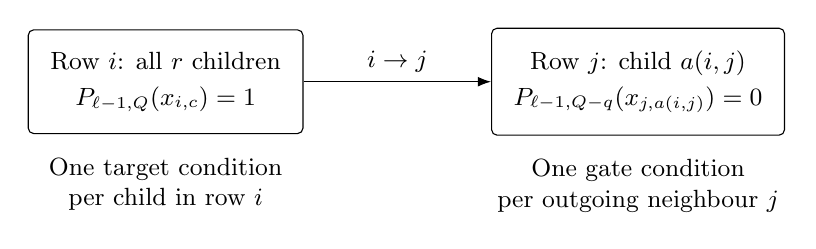
\begin{tikzpicture}[>=Latex, every node/.style={font=\small},
  condition/.style={draw,rounded corners=2pt,inner sep=8pt,align=center}]
 \node[condition] (target) at (0,0)
   {Row \(i\): all \(r\) children\\[2pt]
    \(P_{\ell-1,Q}(x_{i,c})=1\)};
 \node[condition] (gate) at (6,0)
   {Row \(j\): child \(a(i,j)\)\\[2pt]
    \(P_{\ell-1,Q-q}(x_{j,a(i,j)})=0\)};
 \draw[->] (target) -- node[above]{\(i\to j\)} (gate);
 \node[below=5pt of target,align=center] {One target condition\\per child in row \(i\)};
 \node[below=5pt of gate,align=center] {One gate condition\\per outgoing neighbour \(j\)};
\end{tikzpicture}
\caption{One recursive clause. The edge label selects a single child in
each outgoing neighbour's row. Raising \(q\) strengthens the gates;
all targets use the strongest child predicate \(Q\).}
\label{fig:clause}
\end{figure}

\begin{remark}[Smallest example]
For \(d=1\): level \(0\) has \(P_{0,1}\) (radius \(1\)) and \(P_{0,2}\)
(radius \(0\)). At level \(1\) we have \(H=1\), \(Q=2\), and only \(q=1\).
Clause \(i\) says that every child of row \(i\) \emph{equals} a centre, and
that for each edge \(i\to j\) the labelled child of row \(j\) is at distance
at least \(2\) from every centre.
\end{remark}

\subsection{Structure of the clauses}

The following lemma collects the elementary facts used in every counting
argument of Section~\ref{sec:recurrences}. For a predicate list at level
\(\ell\) and indices \(p<p'\), nesting \(P_{\ell,p}\ge P_{\ell,p'}\) is used in
two equivalent forms, which we name:
\begin{itemize}[nosep]
\item[(N1)] \(P_{\ell,p'}(y)=1\ \Longrightarrow\ P_{\ell,p}(y)=1\)
 (acceptance passes to every \emph{smaller} index);
\item[(N0)] \(P_{\ell,p}(y)=0\ \Longrightarrow\ P_{\ell,p'}(y)=0\)
 (rejection passes to every \emph{larger} index).
\end{itemize}
Nesting concerns the predicate index, not the input bits: the predicates are
not monotone in \(x\).

\begin{lemma}\label{lem:structure}
\begin{enumerate}[label=\textup{(\alph*)},ref=\textup{(\alph*)}]
\item\label{it:nest} \textup{(Nesting.)} For every \(0\le\ell\le d\), every
 \(y\in\{0,1\}^{N_\ell}\) and all \(1\le p<p'\le H_\ell\),
 \(P_{\ell,p}(y)\ge P_{\ell,p'}(y)\); that is, \textup{(N1)} and
 \textup{(N0)} hold. Moreover, for \(\ell\ge1\), \(i\in[k]\) and \(q<q'\) in
 \([H_\ell]\): every condition of clause \(i\) that holds at index \(q'\)
 also holds at index \(q\) (the gate for a given edge at index \(q'\)
 implies the gate for the same edge at index \(q\); the targets are
 identical). In particular, clause \(i\) satisfied at index \(q'\) implies
 clause \(i\) satisfied at index \(q\).
\item\label{it:distinct} \textup{(Distinct children.)} Let \(\ell\ge1\) and
 \(i\in[k]\). The children tested by clause \(i\) are the \(r\) target
 children \((i,c)\), \(c\in[r]\), and the \(M^2\) gate children
 \((j,a(i,j))\), \(i\to j\). These \(r+M^2\) children are pairwise distinct
 and do not depend on the index \(q\).
\item\label{it:oneflip} \textup{(One flip, one condition.)} Let \(\ell\ge1\),
 \(x\in\{0,1\}^{N_\ell}\), and let \(e\) be a coordinate, lying in child
 \((j,c)\). For every clause \(i\) and index \(q\), every condition of
 clause \(i\) that does not test child \((j,c)\) has the same truth value
 at \(x\) and at \(x^e\); and at most one condition of clause \(i\) at index
 \(q\) tests child \((j,c)\).
\item\label{it:repair} \textup{(Repair.)} In the situation of
 \ref{it:oneflip}, suppose clause \(i\) at index \(q\) is false at \(x\) and
 true at \(x^e\). Then at \(x\) clause \(i\) has \emph{exactly one} failed
 condition at index \(q\), and this condition tests the child containing
 \(e\).
\end{enumerate}
\end{lemma}
\begin{proof}
\ref{it:nest} By induction on \(\ell\). At level \(0\), \(p<p'\) gives
\(d+1-p>d+1-p'\), so \(D(y)\le d+1-p'\) implies \(D(y)\le d+1-p\). Let
\(\ell\ge1\) and assume nesting at level \(\ell-1\). Let \(q<q'\). The
targets of clause \(i\) do not involve the index. For a gate, \(Q-q'<Q-q\),
so if the gate holds at index \(q'\), i.e.\ \(P_{\ell-1,Q-q'}=0\) on its
child, then (N0) at level \(\ell-1\) gives \(P_{\ell-1,Q-q}=0\) on that
child, i.e.\ the gate holds at index \(q\). Hence clause \(i\) at \(q'\)
implies clause \(i\) at \(q\), and taking the OR over \(i\) gives
\(P_{\ell,q'}\le P_{\ell,q}\).

\ref{it:distinct} Target children lie in row \(i\) at distinct positions.
Gate children lie in rows \(j\ne i\), and there is exactly one gate per
out-neighbour \(j\), so different gates lie in different rows. The list does
not mention \(q\).

\ref{it:oneflip} The strings \(x\) and \(x^e\) agree on every child other
than \((j,c)\), and each condition depends only on the child it tests. The
second assertion is \ref{it:distinct}.

\ref{it:repair} Clause \(i\) is false at \(x\), so it has at least one failed
condition there. Every condition failed at \(x\) holds at \(x^e\), hence
changes truth value, hence tests the child containing \(e\) by
\ref{it:oneflip}; and at most one condition does.
\end{proof}

\section{Profiles, the base level, and blocks at zero}
\label{sec:profiles}

\subsection{Sensitivity profiles}
For \(0\le\ell\le d\) and \(b\in\{0,1\}\), define
\[
 S_{\ell,b}=\max_{\substack{1\le q\le H_\ell,\ x\in\{0,1\}^{N_\ell}\\
                           P_{\ell,q}(x)=b}}
 \bigl|\{e\in[N_\ell]:P_{\ell,q}(x^e)=1-b\}\bigr| ,
\]
\[
 J_{\ell,b}=\max_{\substack{1\le q<q'\le H_\ell,\ x\in\{0,1\}^{N_\ell}\\
                         P_{\ell,q}(x)=P_{\ell,q'}(x)=b}}
 \bigl|\{e\in[N_\ell]:P_{\ell,q}(x^e)=P_{\ell,q'}(x^e)=1-b\}\bigr|.
\]
Thus \(S_{\ell,0}\) bounds the number of flips taking any one predicate of
level \(\ell\) from \(0\) to \(1\), and \(S_{\ell,1}\) those from \(1\) to
\(0\). \(J_{\ell,b}\) bounds the number of flips that move two
\emph{distinct} predicates of level \(\ell\), evaluated at the same input,
simultaneously from \(b\) to \(1-b\). A maximum over no cases is defined to
be zero; in particular \(J_{d,0}=J_{d,1}=0\), since \(H_d=1\).

\subsection{The base level}

The next lemma supplies the initial values for the induction in
Lemma~\ref{lem:quantitative-profiles}.

\begin{lemma}\label{lem:base}
The initial sensitivity profiles satisfy
\begin{equation}\label{eq:base-profile}
 S_{0,0}\le L,\qquad S_{0,1}\le LM,\qquad
 J_{0,0}=J_{0,1}=0.
\end{equation}
\end{lemma}
\begin{proof}
\emph{Step 1 (\(S_{0,0}\le L\)).} Fix \(q\), put \(R=d+1-q\in\{0,\ldots,d\}\),
and let \(x\) satisfy \(P_{0,q}(x)=0\), i.e.\ \(D(x)\ge R+1\). Let \(e\) be a
coordinate with \(P_{0,q}(x^e)=1\), and choose \(j\) with
\(\dist(x^e,z_j)\le R\). Then \(\dist(x,z_j)\le R+1\) by the triangle
inequality, and \(\dist(x,z_j)\ge D(x)\ge R+1\). So \(\dist(x,z_j)=R+1\) and
flipping \(e\) decreased the distance to \(z_j\). Hence \(e\) is one of the
\(R+1\) coordinates in which \(x\) and \(z_j\) differ.

The centre \(z_j\) does not depend on \(e\): if two distinct centres were
both within distance \(R+1\le d+1\) of \(x\), their mutual distance would be
at most \(2d+2<2d+4=2L\), contradicting that distinct centres are at
distance \(2L\). So all successful coordinates \(e\) lie among the same
\(R+1\le d+1\le L\) coordinates.

\emph{Step 2 (\(S_{0,1}\le LM\)).} This is the number of input bits.

\emph{Step 3 (\(D\) is \(1\)-Lipschitz).} For adjacent inputs \(x,y\) and
every \(j\), \(\dist(x,z_j)\le\dist(y,z_j)+1\); taking minima gives
\(D(x)\le D(y)+1\), and by symmetry \(|D(x)-D(y)|\le1\).

\emph{Step 4 (\(J_{0,b}=0\)).} Let \(q<q'\), with radii
\(R=d+1-q\) and \(R'=d+1-q'\), so \(R\ge R'+1\). If both predicates are \(0\)
at \(x\) and both are \(1\) at \(x^e\), then \(D(x)\ge R+1\ge R'+2\) and
\(D(x^e)\le R'\), a change of at least \(2\), contradicting Step~3. If both
are \(1\) at \(x\) and both are \(0\) at \(x^e\), then \(D(x)\le R'\) and
\(D(x^e)\ge R+1\ge R'+2\), again impossible. So no coordinate is counted and
\(J_{0,0}=J_{0,1}=0\).
\end{proof}

\subsection{Disjoint blocks at zero}

The next lemma gives the block-sensitivity lower bound in the proof of
Theorem~\ref{thm:main}. It concerns only the all-zero input.

\begin{lemma}\label{lem:blocks}
At every level \(0\le\ell\le d\), all predicates are zero at the
all-zero input. There are \(Mk^\ell\) pairwise disjoint nonempty blocks
of coordinates, each of size \(Lr^\ell\), such that flipping any one
block at zero makes every predicate at that level equal to one.
\end{lemma}
\begin{proof}
By induction on \(\ell\).

\emph{Level \(0\).} Every centre has exactly \(L\) ones, so \(D(0)=L>d\),
and every radius is at most \(d\); hence all \(P_{0,q}(0)=0\). The \(M\)
blocks \(E_j\) are disjoint, nonempty, of size \(L\), and \(0^{E_j}=z_j\) has
\(D(z_j)=0\), so every \(P_{0,q}(0^{E_j})=1\).

\emph{Level \(\ell\ge1\), assuming level \(\ell-1\).}

\emph{Step 1 (all predicates reject \(0\)).} All children of the all-zero
input are all-zero, so by induction \(P_{\ell-1,Q}\) rejects each of them.
Every clause has \(r\ge1\) targets, all failing. Hence
\(P_{\ell,q}(0)=0\) for every \(q\).

\emph{Step 2 (the blocks).} Let \(B_1,\ldots,B_{Mk^{\ell-1}}\subseteq
[N_{\ell-1}]\) be the block family of level \(\ell-1\). For a row \(i\in[k]\)
and an index \(h\), let \(B_{i,h}\) be the union, over the \(r\) children of
row \(i\), of the copy of \(B_h\) inside that child.

\emph{Step 3 (each \(B_{i,h}\) works).} In \(0^{B_{i,h}}\), each child of row
\(i\) equals \(0^{B_h}\), on which every level-\((\ell-1)\) predicate is
\(1\) by induction; in particular \(P_{\ell-1,Q}\) accepts, so all targets
of clause \(i\) hold. All gate children of clause \(i\) lie in rows other
than \(i\), are still all-zero, and are rejected by every
level-\((\ell-1)\) predicate, so all gates of clause \(i\) hold at every
index \(q\). Thus clause \(i\) is satisfied at every index and
\(P_{\ell,q}(0^{B_{i,h}})=1\) for all \(q\).

\emph{Step 4 (disjointness and counts).} For \(i\ne i'\) the blocks lie in
different rows. For fixed \(i\) and \(h\ne h'\), they are disjoint inside
each child because \(B_h\cap B_{h'}=\emptyset\). There are
\(k\cdot Mk^{\ell-1}=Mk^\ell\) blocks, each nonempty of size
\(r\cdot Lr^{\ell-1}=Lr^\ell\).
\end{proof}

\section{The sensitivity recurrences}
\label{sec:recurrences}

This is the core of the paper. The estimates hold at \emph{every} input, not
only near the all-zero input. They feed
Lemma~\ref{lem:quantitative-profiles}.

\begin{proposition}\label{prop:recurrences}
For \(1\leq \ell\leq d\), write
\(S'_b=S_{\ell-1,b}\) and \(J'_b=J_{\ell-1,b}\).  Then
\begin{equation}\label{eq:recurrences}
\begin{aligned}
 S_{\ell,1}&\leq M^2S'_0+rS'_1,
 &\qquad J_{\ell,1}&\leq M^2J'_0+rS'_1,\\
 S_{\ell,0}&\leq tS'_0+S'_1+3J'_1,
 &\qquad J_{\ell,0}&\leq tS'_0+3J'_1.
\end{aligned}
\end{equation}
\end{proposition}

\paragraph{Plan.}
Steps~A and~B treat flips away from the value \(1\): fix one satisfied
clause and count the flips that break it. Step~C analyses an input where a
predicate is \(0\): it identifies the clauses that are one condition short
(the lists \(\mathcal T\) and \(\mathcal G\)) and bounds their number.
Steps~D and~E then charge each successful flip to a clause in these lists.

\begin{proof}
Fix \(\ell\), and put \(H=H_\ell\), \(Q=H+1=H_{\ell-1}\) as in
\eqref{eq:predicate-definition}. Given an input \(x\) and a coordinate \(e\),
``before'' means at \(x\) and ``after'' means at \(x^e\). ``The value of
\(P_{\ell-1,p}\) on child \((j,c)\)'' means \(P_{\ell-1,p}(x_{j,c})\) before
and \(P_{\ell-1,p}((x^e)_{j,c})\) after.

\medskip\noindent\textbf{Counting rule (R).}
Fix a child \((j,c)\). The coordinates \(e\) of \(x\) inside this child
correspond bijectively to the coordinates of the string \(y=x_{j,c}\), and
flipping \(e\) replaces \(y\) by \(y\) with that coordinate flipped while
leaving all other children unchanged. Applying the definitions of
\(S_{\ell-1,b}\) and \(J_{\ell-1,b}\) to the input \(y\) gives, for
\(b\in\{0,1\}\):
\begin{itemize}[nosep]
\item[(R1)] for every \(p\in[Q]\), at most \(S'_b\) coordinates \(e\) in child
 \((j,c)\) change \(P_{\ell-1,p}\) on that child from \(b\) to \(1-b\);
\item[(R2)] for all \(p<p'\) in \([Q]\), at most \(J'_b\) coordinates \(e\) in
 child \((j,c)\) change \emph{both} \(P_{\ell-1,p}\) and \(P_{\ell-1,p'}\) on
 that child from \(b\) to \(1-b\).
\end{itemize}
A child may be tested by several clauses. This is harmless: we always bound
a set of coordinates by a union of sets, one per clause.

\medskip\noindent\textbf{Step A: \(S_{\ell,1}\le M^2S'_0+rS'_1\).}
Fix \(q\in[H]\) and \(x\) with \(P_{\ell,q}(x)=1\), and fix one clause \(i\)
satisfied at \(x\) at index \(q\). Let \(e\) be a coordinate with
\(P_{\ell,q}(x^e)=0\). Then clause \(i\) is false after, so some condition
of clause \(i\) holds before and fails after; by
Lemma~\ref{lem:structure}\ref{it:oneflip} it tests the child containing
\(e\).
\begin{itemize}[nosep]
\item If it is a gate, then \(P_{\ell-1,Q-q}\) on that gate child changes
 from \(0\) to \(1\). By (R1) each gate child contains at most \(S'_0\)
 such \(e\), and there are \(M^2\) gate children.
\item If it is a target, then \(P_{\ell-1,Q}\) on that target child changes
 from \(1\) to \(0\). By (R1) each target child contains at most \(S'_1\)
 such \(e\), and there are \(r\) target children.
\end{itemize}
So at most \(M^2S'_0+rS'_1\) coordinates \(e\) qualify. As \(q\) and \(x\)
were arbitrary, the bound on \(S_{\ell,1}\) follows.

\medskip\noindent\textbf{Step B: \(J_{\ell,1}\le M^2J'_0+rS'_1\).}
Assume \(H\ge2\) (otherwise \(J_{\ell,1}=0\)). Fix \(q<q'\) in \([H]\) and
\(x\) with \(P_{\ell,q}(x)=P_{\ell,q'}(x)=1\). Fix one clause \(i\) satisfied
at \(x\) at the \emph{larger} index \(q'\). By
Lemma~\ref{lem:structure}\ref{it:nest} it is satisfied at \(x\) at index
\(q\) too. Put
\[
 \gamma=Q-q,\qquad \gamma'=Q-q',\qquad 1\leq \gamma'<\gamma\le Q-1 .
\]
So before the flip, on every gate child of clause \(i\),
\begin{equation}\label{eq:B-before}
 P_{\ell-1,\gamma'}=0\quad\text{(gate holds at index \(q'\))},\qquad
 P_{\ell-1,\gamma}=0\quad\text{(by (N0), as \(\gamma'<\gamma\))}.
\end{equation}
Let \(e\) be a coordinate with \(P_{\ell,q}(x^e)=P_{\ell,q'}(x^e)=0\). We use
only \(P_{\ell,q}(x^e)=0\): every clause, in particular clause \(i\), is
false after at index \(q\). Since clause \(i\) at index \(q\) was true
before, one of its conditions at index \(q\) holds before and fails after,
and it tests the child containing \(e\)
(Lemma~\ref{lem:structure}\ref{it:oneflip}).
\begin{itemize}[nosep]
\item If it is a target: exactly as in Step~A, at most \(rS'_1\) coordinates
 in total.
\item If it is the gate on some gate child: after the flip the gate at
 index \(q\) fails, i.e.\ \(P_{\ell-1,\gamma}=1\) on that child, and then
 (N1) gives \(P_{\ell-1,\gamma'}=1\) on that child. Together with
 \eqref{eq:B-before}, both \(P_{\ell-1,\gamma'}\) and \(P_{\ell-1,\gamma}\)
 change from \(0\) to \(1\). By (R2) each gate child contains at most
 \(J'_0\) such \(e\), and there are \(M^2\) gate children.
\end{itemize}
So at most \(M^2J'_0+rS'_1\) coordinates qualify, which is the bound on
\(J_{\ell,1}\). Steps~A and~B give the first line of~\eqref{eq:recurrences}.

\medskip\noindent\textbf{Step C: the candidate clauses at a zero.}
Fix \(q\in[H]\) and \(x\) with \(P_{\ell,q}(x)=0\). In Step~C, ``fails'' and
``holds'' refer to the input \(x\) and the index \(q\). Define
\begin{align*}
 \mathcal T&=\{\,i\in[k]:\text{clause \(i\) fails exactly one target and no gate}\,\},\\
 \mathcal G&=\{\,i\in[k]:\text{clause \(i\) fails exactly one gate and no target}\,\}.
\end{align*}
These sets depend only on \(x\) and \(q\), not on any flipped coordinate.
For \(W\in\mathcal T\cup\mathcal G\) let \(\kappa(W)\) be the child tested
by the unique failed condition of clause \(W\).

\smallskip\noindent\emph{C1 (every successful flip repairs a candidate).}
Let \(e\) be a coordinate and let \(W\) be a clause satisfied at \(x^e\) at
index \(q\). Then \(W\in\mathcal T\cup\mathcal G\) and \(e\) lies in child
\(\kappa(W)\).

\emph{Proof.} Since \(P_{\ell,q}(x)=0\), clause \(W\) is false at \(x\). By
Lemma~\ref{lem:structure}\ref{it:repair}, clause \(W\) has exactly one
failed condition at \(x\), and it tests the child containing \(e\). That
condition is a target (then \(W\in\mathcal T\)) or a gate (then
\(W\in\mathcal G\)).

\smallskip\noindent\emph{C2 (\(|\mathcal T|\le t-1\)).}
For \(j\in\mathcal T\) let \(m_j\in[r]\) be the position of its unique failed
target, so \(\kappa(j)=(j,m_j)\) and \(P_{\ell-1,Q}(x_{j,c})=1\) for all
\(c\ne m_j\). We claim:
\[
 i,j\in\mathcal T,\ i\to j\quad\Longrightarrow\quad a(i,j)=m_j .
\]
Indeed, clause \(i\) fails no gate, so its gate for the edge \(i\to j\)
holds: \(P_{\ell-1,Q-q}(x_{j,a(i,j)})=0\). Since \(Q-q<Q\), (N0) gives
\(P_{\ell-1,Q}(x_{j,a(i,j)})=0\). That is, the target of clause \(j\) at
position \(a(i,j)\) fails. The only failed target of clause \(j\) is at
position \(m_j\), so \(a(i,j)=m_j\).

If \(|\mathcal T|\ge t\), pick \(I\subseteq\mathcal T\) with \(|I|=t\). The
choices \((m_j)_{j\in I}\) satisfy \(a(i,j)=m_j\) for every edge \(i\to j\)
within \(I\), contradicting Lemma~\ref{lem:labelling}. Hence
\(|\mathcal T|\le t-1\).

\smallskip\noindent\emph{C3 (structure of \(\mathcal G\)).}
\begin{enumerate}[label=\textup{(\roman*)},nosep]
\item \emph{If \(i,j\in\mathcal G\) and \(i\to j\), then the gate of clause
 \(i\) for the edge \(i\to j\) fails, and on its child \((j,a(i,j))\) we
 have \(P_{\ell-1,Q}=1\) and \(P_{\ell-1,Q-q}=1\).} Since
 \(j\in\mathcal G\), clause \(j\) fails no target, so
 \(P_{\ell-1,Q}(x_{j,c})=1\) for every \(c\), in particular for
 \(c=a(i,j)\). Since \(Q-q<Q\), (N1) gives
 \(P_{\ell-1,Q-q}(x_{j,a(i,j)})=1\), which is the failure of that gate.
\item \emph{Each \(i\in\mathcal G\) has at most one out-neighbour in
 \(\mathcal G\).} By (i), distinct out-neighbours in \(\mathcal G\) give
 distinct failed gates of clause \(i\), and clause \(i\) has exactly one
 failed gate.
\item \emph{\(|\mathcal G|\le3\).} The tournament restricted to
 \(\mathcal G\) has \(\binom{|\mathcal G|}{2}\) edges. Each edge leaves
 exactly one vertex, so by (ii) the number of edges is at most
 \(|\mathcal G|\). Thus
 \(|\mathcal G|(|\mathcal G|-1)/2\le|\mathcal G|\), which forces
 \(|\mathcal G|\le3\).
\item \emph{At most one \(i\in\mathcal G\) has no out-neighbour in
 \(\mathcal G\).} Of two distinct vertices of \(\mathcal G\), the edge
 between them leaves one of them.
\end{enumerate}
Call a clause of \(\mathcal G\) with no out-neighbour in \(\mathcal G\)
\emph{exceptional}; by (iv) there is at most one. Every non-exceptional
\(i\in\mathcal G\) has a unique out-neighbour \(j\in\mathcal G\); by (i) its
unique failed gate is the one for \(i\to j\), so
\(\kappa(i)=(j,a(i,j))\) and
\begin{equation}\label{eq:G-before}
 P_{\ell-1,Q-q}=P_{\ell-1,Q}=1\quad\text{on child }\kappa(i)\text{ before the flip.}
\end{equation}
(Examples: if \(\mathcal G=\{i,j\}\) with \(i\to j\), then \(j\) is
exceptional and \(i\) is not; if \(|\mathcal G|=3\), the three vertices form
a directed cycle and none is exceptional.)

\medskip\noindent\textbf{Step D: \(S_{\ell,0}\le tS'_0+S'_1+3J'_1\).}
Keep \(q\), \(x\), \(\mathcal T\), \(\mathcal G\), \(\kappa\) from Step~C.
For \(W\in\mathcal T\cup\mathcal G\) define
\[
 \Phi(W)=\{\,e\text{ in child }\kappa(W):
 \text{clause \(W\) is satisfied at \(x^e\) at index \(q\)}\,\}.
\]
If \(P_{\ell,q}(x^e)=1\), some clause \(W\) is satisfied at \(x^e\), and by C1
\(e\in\Phi(W)\). Hence
\[
 \{e:P_{\ell,q}(x^e)=1\}\subseteq
 \bigcup_{W\in\mathcal T\cup\mathcal G}\Phi(W),
\]
and it suffices to bound each \(|\Phi(W)|\). Let \(e\in\Phi(W)\); then the
unique failed condition of clause \(W\) holds after the flip.
\begin{itemize}[leftmargin=2.2em]
\item[D1.] \(W=j\in\mathcal T\): the target on child \((j,m_j)\) is repaired,
 so \(P_{\ell-1,Q}\) on that child changes from \(0\) to \(1\). By (R1),
 \(|\Phi(j)|\le S'_0\).
\item[D2.] \(W=i\in\mathcal G\) non-exceptional: after the flip the gate on
 \(\kappa(i)\) holds, i.e.\ \(P_{\ell-1,Q-q}=0\) there, and then (N0) gives
 \(P_{\ell-1,Q}=0\) there. By \eqref{eq:G-before} both predicates were \(1\)
 before. The indices \(Q-q\) and \(Q\) are distinct because \(q\ge1\), and
 both lie in \([Q]\). By (R2), \(|\Phi(i)|\le J'_1\). (Such a flip destroys a
 target of the clause of row \(j\). This is irrelevant: we only bound the
 number of coordinates after which clause \(i\) holds.)
\item[D3.] \(W=i\in\mathcal G\) exceptional: the failed gate on \(\kappa(i)\)
 is repaired, so \(P_{\ell-1,Q-q}\) on that child changes from \(1\) to
 \(0\). By (R1), \(|\Phi(i)|\le S'_1\). (Here nothing is known about
 \(P_{\ell-1,Q}\) on \(\kappa(i)\), so (R2) is not available.)
\end{itemize}
By C2 there are at most \(t-1\) clauses of type D1; by C3 there are at most
\(3\) of type D2 and at most \(1\) of type D3. Therefore the number of
successful coordinates is at most
\((t-1)S'_0+3J'_1+S'_1\le tS'_0+S'_1+3J'_1\).

\medskip\noindent\textbf{Step E: \(J_{\ell,0}\le tS'_0+3J'_1\).}
Assume \(H\ge2\). Fix \(q<q'\) in \([H]\) and \(x\) with
\(P_{\ell,q}(x)=P_{\ell,q'}(x)=0\). Form \(\mathcal T\), \(\mathcal G\),
\(\kappa\) exactly as in Step~C for this \(x\) and the \emph{smaller} index
\(q\); C1--C3 apply. Put \(\gamma=Q-q\), \(\gamma'=Q-q'\), so
\(1\le\gamma'<\gamma\le Q-1\). For \(W\in\mathcal T\cup\mathcal G\) define
\[
 \Phi'(W)=\{\,e\text{ in child }\kappa(W):
 \text{clause \(W\) is satisfied at \(x^e\) at index \(q'\)}\,\}.
\]

\emph{E0 (reduction).} Let \(e\) satisfy
\(P_{\ell,q}(x^e)=P_{\ell,q'}(x^e)=1\). Choose a clause \(W\) satisfied at
\(x^e\) at index \(q'\); it exists because \(P_{\ell,q'}(x^e)=1\), and it may
depend on \(e\). By Lemma~\ref{lem:structure}\ref{it:nest}, \(W\) is also
satisfied at \(x^e\) at index \(q\). By C1, \(W\in\mathcal T\cup\mathcal G\)
and \(e\) lies in \(\kappa(W)\). So \(e\in\Phi'(W)\), and
\[
 \{e:P_{\ell,q}(x^e)=P_{\ell,q'}(x^e)=1\}\subseteq
 \bigcup_{W\in\mathcal T\cup\mathcal G}\Phi'(W).
\]

\emph{E1 (\(W=j\in\mathcal T\)).} By
Lemma~\ref{lem:structure}\ref{it:nest}, \(\Phi'(j)\subseteq\Phi(j)\), so
\(|\Phi'(j)|\le S'_0\) by D1.

\emph{E2 (\(W=i\in\mathcal G\), exceptional or not).} The child
\(\kappa(i)\) is the gate child of the unique gate of clause \(i\) that
fails at \(x\) at index \(q\). Hence, before the flip, \(P_{\ell-1,\gamma}=1\)
on \(\kappa(i)\), and (N1) gives \(P_{\ell-1,\gamma'}=1\) on \(\kappa(i)\)
as well. Let \(e\in\Phi'(i)\). After the flip, clause \(i\) holds at index
\(q'\). Its gate for the same edge tests the same child \(\kappa(i)\)
(Lemma~\ref{lem:structure}\ref{it:distinct}), so
\(P_{\ell-1,\gamma'}=0\) on \(\kappa(i)\) after, and (N0) gives
\(P_{\ell-1,\gamma}=0\) there. Thus the two distinct predicates
\(P_{\ell-1,\gamma'}\) and \(P_{\ell-1,\gamma}\) both change from \(1\) to
\(0\) on \(\kappa(i)\), and (R2) gives \(|\Phi'(i)|\le J'_1\).

\emph{Why no \(S'_1\) term appears here.} In D2 the second predicate was
\(P_{\ell-1,Q}\), whose initial value \(1\) came from the row of
\(\kappa(i)\) belonging to \(\mathcal G\); this was unavailable for the
exceptional clause, which is why D3 used \(S'_1\). In E2 the second
predicate is \(P_{\ell-1,\gamma'}\), supplied by the second parent index
\(q'\). Its initial value \(1\) follows from nesting alone, with no
information about targets. So E2 covers the exceptional clause too.

\emph{E3 (sum).} With \(|\mathcal T|\le t-1\) and \(|\mathcal G|\le3\), the
number of joint-success coordinates is at most
\((t-1)S'_0+3J'_1\le tS'_0+3J'_1\).

\medskip\noindent\textbf{Step F: conclusion.}
Steps A, B, D, E hold for every admissible input and every index or pair of
indices, so taking maxima gives \eqref{eq:recurrences}. If \(H=1\) there is
no pair \(q<q'\), and \(J_{\ell,0}=J_{\ell,1}=0\) by the empty-maximum
convention, so the two joint inequalities hold trivially.
\end{proof}

\begin{remark}[The source's formulation of Step~E]
The source adds two observations which are true but not needed for the
count above. First, a witness \(W\) as in E0 had exactly one failed
condition at \(x\) at index \(q'\) as well: since \(P_{\ell,q'}(x)=0\),
clause \(W\) is false at \(x\) at index \(q'\) and true at \(x^e\), so
Lemma~\ref{lem:structure}\ref{it:repair} applies at index \(q'\). That
condition tests the child containing \(e\), i.e.\ \(\kappa(W)\). Second, a
clause of \(\mathcal T\cup\mathcal G\) with two or more failed conditions at
index \(q'\) is therefore never a witness; for it \(\Phi'(W)=\emptyset\),
which only helps the upper bound.
\end{remark}

\section{Quantitative bounds and the proof of Theorem~\ref{thm:main}}
\label{sec:separation}

\subsection{Solving the recurrences}

The dominant terms \(M^2S'_0\) and \(S'_1\) in
Proposition~\ref{prop:recurrences} suggest normalising \(S_{\ell,b}\) by
\(M^{\ell+b}\). The next lemma is used in the proof of
Theorem~\ref{thm:main} at \(\ell=d\).

\begin{lemma}
\label{lem:quantitative-profiles}
Suppose that \(d\geq 1\) and \(M\geq 9^{d+1}\).
For every \(0\leq\ell\leq d\) and \(b\in\{0,1\}\), the predicates of the
construction satisfy
\[
  S_{\ell,b}\leq 2L M^{\ell+b}.
\]
\end{lemma}

\paragraph{Plan.}
Normalise the four recurrences into two (Step~2), dominate the normalised
quantities by explicit comparison sequences (Step~4), and bound those by
induction (Step~5). The hypothesis \(M\ge9^{d+1}\) enters only through the
bound \(\epsilon\le2/3^{d+1}\) of Step~3, which is used only at the end of
Step~5.

\begin{proof}
\emph{Step 1 (normalised quantities).} Define
\[
 u_\ell=\max_{b\in\{0,1\}}\frac{S_{\ell,b}}{M^{\ell+b}},
 \qquad
 v_\ell=\max_{b\in\{0,1\}}\frac{J_{\ell,b}}{M^{\ell+b}},
 \qquad
 \epsilon=\frac{\max(r,t)}{M}.
\]
Note that \(\epsilon\) is determined by \(M\); it is not a free parameter.
By~\eqref{eq:base-profile}, \(S_{0,0}/M^0\le L\) and \(S_{0,1}/M^1\le L\), so
\(u_0\leq L\), and \(v_0=0\).

\emph{Step 2 (normalised recurrences).} Let \(1\leq\ell\leq d\) and write
\(u=u_{\ell-1}\), \(v=v_{\ell-1}\). By definition,
\(S'_b\le u\,M^{\ell-1+b}\) and \(J'_b\le v\,M^{\ell-1+b}\). Substituting into
\eqref{eq:recurrences}:
\begin{align*}
 S_{\ell,1}&\le M^2\cdot uM^{\ell-1}+r\cdot uM^{\ell}
   =M^{\ell+1}\Bigl(1+\frac rM\Bigr)u,\\
 S_{\ell,0}&\le t\cdot uM^{\ell-1}+uM^{\ell}+3vM^{\ell}
   =M^{\ell}\Bigl[\Bigl(1+\frac tM\Bigr)u+3v\Bigr],\\
 J_{\ell,1}&\le M^2\cdot vM^{\ell-1}+r\cdot uM^{\ell}
   =M^{\ell+1}\Bigl(\frac rM\,u+v\Bigr),\\
 J_{\ell,0}&\le t\cdot uM^{\ell-1}+3vM^{\ell}
   =M^{\ell}\Bigl(\frac tM\,u+3v\Bigr).
\end{align*}
Dividing by \(M^{\ell+1}\), \(M^\ell\), \(M^{\ell+1}\), \(M^\ell\)
respectively, and using \(r/M\le\epsilon\), \(t/M\le\epsilon\),
\(v\le3v\), we get
\begin{equation}
\label{eq:normalized-recurrences}
 \begin{split}
  u_\ell&\leq (1+\epsilon)u_{\ell-1}+3v_{\ell-1},\\
  v_\ell&\leq \epsilon u_{\ell-1}+3v_{\ell-1}.
 \end{split}
\end{equation}

\emph{Step 3 (size of \(\epsilon\)).} Since \(d\ge1\), \(M\geq81\), so
\(\sqrt M\ge9\). Then \(r=\lceil\sqrt M\rceil\leq\sqrt M+1\le2\sqrt M\) and
\(t=16\leq 18\le 2\sqrt M\). Hence, using \(\sqrt M\ge 3^{d+1}\),
\begin{equation}
\label{eq:epsilon-choice}
 \epsilon\leq\frac{2\sqrt M}{M}=\frac{2}{\sqrt M}\leq\frac{2}{3^{d+1}}.
\end{equation}

\emph{Step 4 (comparison sequences).} Let \(U_0=L\), \(V_0=0\), and for
\(\ell\ge1\)
\[
 U_\ell=(1+\epsilon)U_{\ell-1}+3V_{\ell-1},
 \qquad
 V_\ell=\epsilon U_{\ell-1}+3V_{\ell-1}.
\]
All coefficients are nonnegative, \(u_0\le U_0\) and \(v_0\le V_0\), so
\eqref{eq:normalized-recurrences} gives \(u_\ell\leq U_\ell\) and
\(v_\ell\leq V_\ell\) for \(0\le\ell\le d\) by induction on \(\ell\).

\emph{Step 5 (bounding the comparison sequences).} We prove by strong
induction that, for \(0\leq\ell\leq d\),
\begin{equation}
\label{eq:comparison-bounds}
 U_\ell\leq2L,
 \qquad
 V_\ell\leq\epsilon L(3^\ell-1).
\end{equation}
At \(\ell=0\): \(U_0=L\le 2L\) and \(V_0=0\). Let \(1\leq\ell\leq d\) and
assume \eqref{eq:comparison-bounds} at every index \(j<\ell\).

\emph{Bound on \(V_\ell\).} Using the bounds at \(\ell-1\),
\[
 V_\ell=\epsilon U_{\ell-1}+3V_{\ell-1}
 \leq 2\epsilon L+3\epsilon L(3^{\ell-1}-1)
 =\epsilon L(2+3^\ell-3)=\epsilon L(3^\ell-1).
\]

\emph{Bound on \(U_\ell\).} The recursion says
\(U_{j+1}-U_{j}=\epsilon U_{j}+3V_{j}\). Summing over \(j=0,\ldots,\ell-1\)
and using \eqref{eq:comparison-bounds} at the indices \(j<\ell\),
\begin{align*}
 U_\ell
 &=L+\sum_{j=0}^{\ell-1}(\epsilon U_j+3V_j)
 \leq L+2\epsilon L\ell
          +3\epsilon L\sum_{j=0}^{\ell-1}(3^j-1).
\end{align*}
Since \(\sum_{j=0}^{\ell-1}(3^j-1)=\frac{3^\ell-1}{2}-\ell\), the right-hand
side equals
\[
 L+\epsilon L\Bigl[2\ell+\tfrac32(3^\ell-1)-3\ell\Bigr]
 =L+\epsilon L\Bigl[\tfrac32(3^\ell-1)-\ell\Bigr].
\]
The bracket is positive (it is at least \(3\ell-\ell\), because
\(3^\ell-1\ge2\ell\)). By \eqref{eq:epsilon-choice} and \(\ell\le d\),
\[
 \epsilon\Bigl[\tfrac32(3^\ell-1)-\ell\Bigr]
 \leq\frac{2}{3^{d+1}}\cdot\frac{3^{\ell+1}-3-2\ell}{2}
 =\frac{3^{\ell+1}-3-2\ell}{3^{d+1}}
 <\frac{3^{\ell+1}}{3^{d+1}}\le1 .
\]
Hence \(U_\ell<L+L=2L\). This completes the induction.

\emph{Step 6.} By Steps 4 and 5, \(u_\ell\le U_\ell\leq2L\), i.e.\
\(S_{\ell,b}\le 2LM^{\ell+b}\) for both \(b\).
\end{proof}

\subsection{Proof of Theorem~\ref{thm:main}}

\begin{proof}[Proof of Theorem~\ref{thm:main}]
Fix an integer \(d\geq1\) and an integer \(M\geq9^{d+1}\), fix a tournament
and a labelling as in Section~\ref{sec:construction}
(Lemma~\ref{lem:labelling}), and form the predicates \(P_{\ell,q}\).

\emph{Step 1 (the function).} Let \(f\) be the OR of \(M\) disjoint copies of
\(P_{d,1}\): the input is a tuple \((y^{(1)},\ldots,y^{(M)})\) of strings in
\(\{0,1\}^{N_d}\), and \(f=1\) iff \(P_{d,1}(y^{(c)})=1\) for some \(c\). Each
copy has \(N_d=LM(kr)^d\) bits, so \(f\) is a total Boolean function on
\begin{equation}
\label{eq:final-dimension}
 n=LM^2(kr)^d
\end{equation}
bits. By Lemma~\ref{lem:blocks} with \(\ell=d\), \(P_{d,1}(0)=0\), so
\(f(0)=0\).

\emph{Step 2 (sensitivity).} Let \(x\) be an input and \(e\) a coordinate;
flipping \(e\) changes exactly one copy.
\begin{itemize}[nosep]
\item If \(f(x)=0\), every copy rejects, and \(f(x^e)=1\) iff the copy
 containing \(e\) accepts after the flip. Each copy contains at most
 \(S_{d,0}\) such coordinates, so \(s(f,x)\le MS_{d,0}\).
\item If \(f(x)=1\) and at least two copies accept, then after any single
 flip some copy still accepts, so \(s(f,x)=0\).
\item If \(f(x)=1\) and exactly one copy accepts, a sensitive coordinate
 must lie in that copy and turn it from \(1\) to \(0\), so
 \(s(f,x)\le S_{d,1}\).
\end{itemize}
Lemma~\ref{lem:quantitative-profiles} gives \(MS_{d,0}\le M\cdot2LM^{d}\) and
\(S_{d,1}\le 2LM^{d+1}\), hence
\begin{equation}
\label{eq:final-sensitivity}
 s(f)\leq\max\{M S_{d,0},S_{d,1}\}
       \leq2L M^{d+1}.
\end{equation}

\emph{Step 3 (block sensitivity at zero).} By Lemma~\ref{lem:blocks} with
\(\ell=d\), there are \(Mk^d\) pairwise disjoint nonempty blocks in
\([N_d]\), each of which turns \(P_{d,1}\) from \(0\) to \(1\) when flipped
at the all-zero input. Place this family in each of the \(M\) copies. The
resulting \(M^2k^d\) blocks are pairwise disjoint, and flipping any one of
them at \(0\) makes one copy accept, so \(f\) becomes \(1\ne f(0)\). Thus
\begin{equation}
\label{eq:final-block-sensitivity}
 \bs(f,0)\geq M^2k^d .
\end{equation}
In particular \(f\) is nonconstant. Hence \(s(f)>0\): the hypercube is
connected, so a nonconstant function differs across some edge.

\emph{Step 4 (ratio).} Combining \eqref{eq:final-sensitivity} and
\eqref{eq:final-block-sensitivity}, and using \(k/M^2=2+1/M^2\ge2\) and
\(L=d+2\),
\begin{equation}
\label{eq:ratio-separation}
 \frac{\bs(f)}{s(f)^2}
 \geq\frac{\bs(f,0)}{s(f)^2}
 \geq\frac{M^2k^d}{4L^2M^{2d+2}}
 =\frac{(k/M^2)^d}{4L^2}
 \geq\frac{2^d}{4(d+2)^2}.
\end{equation}
This is the second assertion of the theorem.

\emph{Step 5 (arbitrary \(C\)).} The right-hand side of
\eqref{eq:ratio-separation} tends to infinity with \(d\). Given \(C>0\),
choose \(d\) with \(2^d/(4(d+2)^2)>C\), then \(M\ge 9^{d+1}\), then the
labelling, and form \(f\). Then \(\bs(f)>C\,s(f)^2\).
\end{proof}

\section{A fixed exponent by composition}
\label{sec:composition}

The construction supplies a fixed seed whose block sensitivity at zero
exceeds the square of its sensitivity; iterated composition of the seed
gives Corollary~\ref{cor:power-separation}. The next lemma contains the two
composition facts needed.

\begin{lemma}
\label{lem:composition}
Let \(f:\{0,1\}^{n_1}\to\{0,1\}\) and
\(g:\{0,1\}^{n_2}\to\{0,1\}\) be total Boolean functions.
Their disjoint composition is the function on \(n_1n_2\) bits defined by
\[
 (f\circ g)(x_1,\ldots,x_{n_1})
   =f\bigl(g(x_1),\ldots,g(x_{n_1})\bigr),
 \qquad x_i\in\{0,1\}^{n_2}.
\]
Then
\[
 s(f\circ g)\leq s(f)s(g).
\]
If \(g(0)=0\), then \((f\circ g)(0)=f(0)\) and
\[
 \bs(f\circ g,0)\geq\bs(f,0)\bs(g,0).
\]
More explicitly, any disjoint families of \(p\) and \(p'\) blocks sensitive
at zero for \(f\) and \(g\), respectively, yield a disjoint family of
\(pp'\) blocks sensitive at zero for \(f\circ g\).
\end{lemma}

\begin{proof}
Identify the coordinates of the composition with \([n_1]\times[n_2]\):
coordinate \((i,e)\) is coordinate \(e\) of the block \(x_i\).

\emph{Sensitivity.} Fix \(x=(x_1,\ldots,x_{n_1})\) and put
\(w=(g(x_1),\ldots,g(x_{n_1}))\in\{0,1\}^{n_1}\), so
\((f\circ g)(x)=f(w)\). Flipping coordinate \((i,e)\) replaces \(x_i\) by
\(x_i^{e}\) and changes nothing else. If \(g(x_i^e)=g(x_i)\), the outer
string is still \(w\) and the value is unchanged. If
\(g(x_i^e)\ne g(x_i)\), the outer string becomes \(w^{i}\), and the value
changes iff \(f(w^{i})\ne f(w)\). So \((i,e)\) is sensitive for \(f\circ g\)
at \(x\) exactly when \(e\) is sensitive for \(g\) at \(x_i\) and \(i\) is
sensitive for \(f\) at \(w\). Therefore
\[
 s(f\circ g,x)
   =\sum_{i:\,f(w^{i})\ne f(w)}s(g,x_i)
   \leq s(f,w)\,s(g)
   \leq s(f)s(g).
\]

\emph{Blocks at zero.} Suppose \(g(0)=0\). Then
\((f\circ g)(0)=f(g(0),\ldots,g(0))=f(0)\). Let
\(X_1,\ldots,X_p\subseteq[n_1]\) be pairwise disjoint sensitive blocks for
\(f\) at \(0\), and \(Y_1,\ldots,Y_{p'}\subseteq[n_2]\) pairwise disjoint
sensitive blocks for \(g\) at \(0\). For \(1\leq s\leq p\) and
\(1\leq s'\leq p'\) set
\[
 Z_{s,s'}=X_s\times Y_{s'}\subseteq[n_1]\times[n_2].
\]
\begin{itemize}[nosep]
\item \emph{Nonempty and pairwise disjoint.} Each factor is nonempty. If
 \((s,s')\ne(\sigma,\sigma')\), then either \(s\ne\sigma\) and
 \(X_s\cap X_\sigma=\emptyset\), or \(s=\sigma\), \(s'\ne\sigma'\) and
 \(Y_{s'}\cap Y_{\sigma'}=\emptyset\); in both cases the products are
 disjoint.
\item \emph{Sensitive.} In \(0^{Z_{s,s'}}\), the block \(x_i\) equals
 \(0^{Y_{s'}}\) for \(i\in X_s\) and equals \(0\) for \(i\notin X_s\). Since
 \(g(0)=0\) and \(Y_{s'}\) is sensitive for \(g\) at \(0\),
 \(g(0^{Y_{s'}})=1\). So the outer string is \(1\) exactly on \(X_s\), i.e.\
 it is the indicator string \(0^{X_s}\) of \(X_s\). Since \(X_s\) is
 sensitive for \(f\) at \(0\), \(f(0^{X_s})\ne f(0)=(f\circ g)(0)\).
\end{itemize}
So the \(pp'\) sets \(Z_{s,s'}\) are pairwise disjoint sensitive blocks for
\(f\circ g\) at \(0\). Taking \(p=\bs(f,0)\) and \(p'=\bs(g,0)\) gives the
inequality; if either is zero it is trivial.
\end{proof}

\begin{proof}[Proof of Corollary~\ref{cor:power-separation}]
\emph{Step 1 (the seed).} Fix \(d=9\), choose an integer \(M\geq9^{10}\) and
an admissible labelling, and let \(f\) be the function constructed in the
proof of Theorem~\ref{thm:main} for these parameters. Here \(L=11\) and
\(k=2M^2+1\). Put
\[
 A=22M^{10},\qquad B=M^2k^9.
\]
By \eqref{eq:final-sensitivity}, \(s(f)\le 2\cdot11\cdot M^{10}=A\); by
\eqref{eq:final-block-sensitivity}, \(\bs(f,0)\geq B\); and \(f(0)=0\)
(Step~1 of that proof).

\emph{Step 2 (the exponent).} Since \(k/M^2\ge2\),
\[
 \frac{B}{A^2}
   =\frac{M^2k^9}{484\,M^{20}}
   =\frac{(k/M^2)^9}{484}
   \geq\frac{2^9}{484}
   =\frac{128}{121}>1.
\]
Also \(A>1\). Hence \(B>A^2>1\) and
\[
 \alpha=\frac{\log B}{\log A}>2 .
\]
This \(\alpha\) depends on the chosen \(M\) and is fixed once \(M\) is.
By definition, \(A^\alpha=B\).

\emph{Step 3 (iteration).} Set \(F_1=f\) and
\(F_{\nu+1}=f\circ F_\nu\) for \(\nu\ge1\). With \(n\) as in
\eqref{eq:final-dimension}, \(F_\nu\) is a total function on \(n^\nu\) bits.
We show by induction on \(\nu\) that
\[
 F_\nu(0)=0,\qquad s(F_\nu)\leq A^\nu,
 \qquad
 \bs(F_\nu,0)\geq B^\nu.
\]
For \(\nu=1\) this is Step~1. If it holds for \(\nu\), apply
Lemma~\ref{lem:composition} with outer function \(f\) and inner function
\(g=F_\nu\), which satisfies \(g(0)=0\):
\(F_{\nu+1}(0)=f(0)=0\),
\(s(F_{\nu+1})\le s(f)s(F_\nu)\le A\cdot A^\nu\), and
\(\bs(F_{\nu+1},0)\ge\bs(f,0)\bs(F_\nu,0)\ge B\cdot B^\nu\).

\emph{Step 4 (conclusions).} Since \(\bs(F_\nu,0)\ge B^\nu\ge1\), there is a
block whose flip at \(0\) changes \(F_\nu\), so \(F_\nu\) is nonconstant.
Since \(B>1\), \(\bs(F_\nu,0)\to\infty\). Since \(t\mapsto t^\alpha\) is
increasing on \([0,\infty)\) and \(A^\alpha=B\),
\[
 s(F_\nu)^\alpha\leq (A^{\nu})^{\alpha}=B^\nu\leq\bs(F_\nu,0).
\]
Finally, \(s(F_\nu)>0\) because \(F_\nu\) is nonconstant, and the same
estimates give the explicit ratio bound
\[
 \frac{\bs(F_\nu)}{s(F_\nu)^2}
 \geq\frac{\bs(F_\nu,0)}{s(F_\nu)^2}
 \geq\left(\frac{B}{A^2}\right)^\nu
 \geq\left(\frac{128}{121}\right)^\nu.\qedhere
\]
\end{proof}

\section{Verification checklist}
\label{sec:checklist}

Every step above was checked while writing and no step is marked as
unverified. The historical statements of Section~1.2 were not checked and
are not used. A sceptical reader should examine the following first.

\begin{enumerate}[leftmargin=2em]
\item \textbf{One flip repairs exactly one failed condition}
 (Lemma~\ref{lem:structure}\ref{it:distinct}--\ref{it:repair}). Everything
 in Section~\ref{sec:recurrences} rests on a clause testing each child at
 most once. Check that gate children of one clause lie in distinct rows,
 all different from the target row.
\item \textbf{Directions of nesting.} (N1)/(N0) are applied to the child
 indices \(Q-q<Q\) and \(\gamma'=Q-q'<\gamma=Q-q\). Check each use: Step~B
 (\eqref{eq:B-before} and the line after), C2 (a passing gate forces a
 failed target), C3(i) (a satisfied target forces a failed gate), D2, E2.
\item \textbf{\(|\mathcal T|\le15\)} (Step~C2 with
 Lemma~\ref{lem:labelling}). Check that the derived relation
 \(a(i,j)=m_j\) is exactly the configuration excluded by the lemma, and
 the arithmetic \(\binom{16}{2}=120\), \(k^{16}r^{16-120}\le3^{16}M^{-20}<1\).
\item \textbf{\(|\mathcal G|\le3\) and the charges} (Steps~C3, D2, D3). Check
 that only non-exceptional clauses use \eqref{eq:G-before}, that at most
 one clause is exceptional, and that the total is \(S'_1+3J'_1\).
\item \textbf{No \(S'_1\) term in \(J_{\ell,0}\)} (Step~E2). Check that the
 initial values \(P_{\ell-1,\gamma}=P_{\ell-1,\gamma'}=1\) use only the
 failed gate at index \(q\) and nesting, and that the witness is chosen at
 the larger index \(q'\) (Step~E0).
\item \textbf{Powers of \(M\) in the normalisation} (Step~2 of
 Lemma~\ref{lem:quantitative-profiles}), and the base values
 \(u_0\le L\), \(v_0=0\) from Lemma~\ref{lem:base} (in particular Step~4
 there, \(J_{0,b}=0\)).
\item \textbf{The induction \(U_\ell<2L\)} (Step~5 of
 Lemma~\ref{lem:quantitative-profiles}). This is the only place where
 \(M\ge9^{d+1}\) is used, via \eqref{eq:epsilon-choice} and \(\ell\le d\).
\item \textbf{The final count} (proof of Theorem~\ref{thm:main}). Check
 \(s(f)\le\max\{MS_{d,0},S_{d,1}\}\), \(\bs(f,0)\ge M^2k^d\) from
 Lemma~\ref{lem:blocks}, and \(k/M^2\ge2\) in
 \eqref{eq:ratio-separation}.
\item \textbf{Composition} (Lemma~\ref{lem:composition}). Check that the
 block bound is only claimed at the all-zero input and needs \(g(0)=0\),
 which the induction in the Corollary maintains, and that
 \(2^9/484=128/121>1\).
\end{enumerate}

\bibliographystyle{alpha}
\bibliography{references}
\end{document}
